% !TEX program = pdflatex
% !TEX encoding = UTF-8
% !TEX spellcheck = en_US
\documentclass[12pt]{article}

\usepackage[margin=1in]{geometry}
\usepackage[utf8]{inputenc}
\usepackage{amsmath,amsthm,amssymb}
\usepackage{graphicx}
\usepackage{hyperref} % Uso de links
\usepackage[version=4]{mhchem}
\usepackage{siunitx}
\usepackage{titlesec}
\usepackage{booktabs}
\usepackage{enumerate}
\usepackage{bm}
\usepackage{miller}
\usepackage{datetime}

\titleformat{\subsection}
  {\normalfont\large\bfseries}{}{0em}{}

\settimeformat{hhmmsstime}

\setlength{\parindent}{0em}

\DeclareMathOperator{\sech}{sech}

\begin{document}

% --------------------------------------------------------------
%                         Start here
% --------------------------------------------------------------

\title{Mechanical Properties of Materials (MSAE 4215), Spring 2019\\ Homework 6 Solutions}
\author{Qi Zhang}
\date{\today, \currenttime}

\maketitle

\tableofcontents
\listoffigures
\listoftables

\section{Problems}
Please track the time above to see whether this file is updated.

\subsection{7.3}
Determine the mode profile and resonant frequencies for a bar which is \textit{clamped}
at both ends, i.e. cannot be displaced in any direction, and fixed in both $x$ and $y$.

\textbf{Solutions:}

A general solution of the equation
\begin{equation}
  \frac{ \partial^4 y }{ \partial x^4 } + \frac{ 1 }{ D } \frac{ \partial^2 y }{ \partial t^2 } = 0
\end{equation}
has the form of
\begin{equation}
  y_n(x) = A_0 \cos k_n x + A_1 \cosh k_n x + B_0 \sin k_n x + B_1 \sinh k_n x,
\end{equation}
where $A$'s and $B$'s are the constants to be solved, and $n \in \mathbb{N}$ is
the label of the $n$th mode.
For a \emph{doubly-clamped beam}, we usually set the boundary conditions to be
\begin{align}
  y(0)  & = y(L) = 0,  \\
  y'(0) & = y'(L) = 0,
\end{align}
where $y = 0$ tells the position of the beam's ends,
and $y' = 0$ says that the beam at the wall is horizontal.

Apply the BCs, we have
\begin{equation}\label{eq:bcssimply}
  \begin{aligned}
    A_0 + A_1                                                            & = 0, \\
    A_0 \cos k_n L + A_1 \cosh k_n L + B_0 \sin k_n L + B_1 \sinh k_n L  & =0,  \\
    B0 + B1                                                              & = 0, \\
    -A_0 \sin k_n L + A_1 \sinh k_n L + B_0 \cos k_n L + B_1 \cosh k_n L & =0.
  \end{aligned}
\end{equation}
Simplify \eqref{eq:bcssimply},
\begin{align}
  \mathrm{ M } \bm{C}       & = \bm{0}, \label{eq:linsys} \\
  \begin{bmatrix}
    \sin k_n L + \sinh k_n L  & -\cos k_n L + \cosh k_n L \\
    -\cos k_n L + \cosh k_n L & -\sin k_n L + \sinh k_n L
  \end{bmatrix}
  \begin{bmatrix}
    A_1 \\
    B_1
  \end{bmatrix} & = \bm{0}.
\end{align}
To let \eqref{eq:linsys} have nonzero solutions,
the determinant of $\mathrm{ M }$ must be zero, i.e.,
\begin{equation}
  \cos ( k_n L ) \cosh ( k_n L ) = 1.
\end{equation}
Solutions are found for approximately
\begin{equation}
  k_n L = \frac{ 3 }{ 2 } \pi, \frac{ 5 }{ 2 } \pi, \frac{ 7 }{ 2 }\pi, \ldots
\end{equation}

\subsection{7.4}
An earthquake strikes the San Francisco Bay Area;
how long does it take for the tremors to be felt in Los Angeles, \SI{600}{\kilo\meter} away?
Assume that the elastic waves propagate as through bulk (not surface) rock with density
of \SI{2.65}{\gram \per \cubic \centi \meter} and Young's modulus of \SI{10}{\giga\pascal}.
Calculate for the P- (primary) wave due to compression and the
S- (secondary) wave due to shear, assuming a poisson ratio of $\nu= 0.25$.

\textbf{Solutions:}

The P-wave modulus is
\begin{equation}
  M = \frac{ E (1 - \nu) }{ 1 - \nu - 2 \nu^2 } = \SI{12}{\giga\pascal}.
\end{equation}
And the shear modulus is
\begin{equation}
  \mu = \frac{ E }{ 2 ( 1 + \nu ) } = \SI{4}{\giga\pascal}.
\end{equation}
So,
\begin{align}
  v_l = \sqrt{\frac{ M }{ \rho }}   & = \SI{2127.98}{\meter\per\second}, \\
  v_t = \sqrt{\frac{ \mu }{ \rho }} & = \SI{1228.59}{\meter\per\second}.
\end{align}
Thus,
\begin{align}
  t_l & = \frac{ d }{ v_l } = \SI{281.96}{\second}, \\
  t_t & = \frac{ d }{ v_t } = \SI{488.36}{\second}.
\end{align}

\subsection{7.5}
Compare longitudinal wave velocities in a single crystal of \ce{Ag} for elastic wave
propagation along the \hkl[100] and \hkl[110] directions.  Is there a directional dependence of the velocity?
Why or why not?

\textbf{Solutions:}

Solid \ce{Ag} has a face-centred cubic (fcc) lattice. So we could use
equations in section $7.2.2$.

For direction \hkl[100], the $3$ sound velocities are
\begin{align}
  v_l & = \sqrt{\frac{ c_{11} }{ \rho }},        \\
  v_t & = v_t' = \sqrt{\frac{ c_{44} }{ \rho }}.
\end{align}
The three corresponding eigenvectors are \hkl[100], \hkl[010] and \hkl[001].
Thus for a wave propagating the $x$ axis, we have a longitudinal wave with particle displacement along the
$x$ axis, and two identical but independent transverse waves with particle displacement along $y$ and $z$ axes.

For direction \hkl[110], the $3$ sound velocities are
\begin{align}
  v_l  & = \sqrt{\frac{ c_{11} + c_{12} + 2 c_{44} }{ 2 \rho }}, & \text{atomic displacement along \hkl[110]},   \\
  v_t  & = \sqrt{\frac{ c_{44} }{ \rho }},                       & \text{ atomic displacement along \hkl[001]}   \\
  v_t' & = \sqrt{\frac{ c_{11} - c_{12} }{ 2 \rho }},            & \text{ atomic displacement along \hkl[-110]}.
\end{align}

For direction \hkl[111], the $3$ sound velocities are
\begin{align}
  v_l  & = \sqrt{\frac{ c_{11} + 2 c_{12} + 4 c_{44} }{ 3 \rho }}, & \text{atomic displacement along \hkl[111]},    \\
  v_t  & = \sqrt{\frac{ c_{11} - c_{12} + c_{44} }{ 3 \rho }},     & \text{ atomic displacement along \hkl[-110]}   \\
  v_t' & = \sqrt{\frac{ c_{11} - c_{12} + c_{44} }{ 3 \rho }},     & \text{ atomic displacement along \hkl[-1-12]}.
\end{align}
Yes, usually there will be a directional dependence of the velocities,
because $c_{11}$, $c_{12}$ and $c_{44}$ may change in different directions, just as what we see in section $6.5$.

\subsection{8.1}
Compare the effective Young's modulus for a $10\%$ volume fraction of hard material $A$ in a matrix of soft material $B$, $E_A=10 E_B$, in two geometries:
\begin{itemize}
  \item Fiber geometry (long axes of fibers along stress)
  \item Plate geometry (composition modulation in direction of primary stress), neglecting Poisson contraction
  \item Plate geometry (composition modulation in direction of primary stress), including Poisson contraction. Take $\nu_A= 0.3$, $\nu_B= 0.45$.
\end{itemize}

\textbf{Solutions:}
\begin{itemize}
  \item Using equation $(8.1)$,
        \begin{equation}
          E = V_A E_A + V_B E_B = 0.1 \times 10 E_B + 0.9 E_B = 1.9 E_B.
        \end{equation}

  \item Using equation $(8.2)$,
        \begin{equation}
          E = \frac{ 1 }{ \frac{ V_A }{ E_A } + \frac{ V_B }{ E_B } }
          = \frac{ 100 }{ 91 } E_B.
        \end{equation}

  \item Using equation $(8.17)$,
        \begin{equation}
          E^{-1} = \frac{V_A}{E_A}+\frac{V_B}{E_B}- \frac{2 V_A V_B}{E_A E_B}\frac{\left(\nu_A E_B-\nu_B E_A\right)^2}{V_A E_A\left(1- \nu_B\right)+ V_B E_B\left(1 - \nu_A\right)}
          \approx 0.64 / E_B,
        \end{equation}
        so $E \approx 1.56 E_B$.
\end{itemize}

\subsection{8.2}
Derive a relationship for the Young's modulus of plates in the $x_1 - x_2$ plane,
$\sigma_1/\epsilon_1$ where the primary stress $\sigma_1$ is applied along one of
the in-plane directions of the plate. Express your answer in terms of the volume
fractions $V_A$, $V_B$ and isotropic elastic constants $E_A, E_B, \nu_A, \nu_B$.

\textbf{Solutions:}

In direction $\hat{\bm{x}}_1$, we have fibre-like tension. So
\begin{equation}\label{eq:sg11}
  \sigma_{1} = V_A \sigma_{1A} + V_B \sigma_{1B},
\end{equation}
where $\sigma_{1}$ denotes the total stress on that direction, and
$V_A$, $V_B$ are the volume fractions of $A$ and $B$, respectively.
This is an isostrain case, so
\begin{equation}
  \varepsilon_{1A} = \varepsilon_{1B} = \varepsilon_{1},
\end{equation}
where
\begin{align}
  \varepsilon_{1A} & = \frac{ \sigma_{1A} }{ E_A } - \frac{ \nu_A }{ E_A } (\sigma_{2A} + \sigma_{3A}), \\
  \varepsilon_{1B} & = \frac{ \sigma_{1B} }{ E_B } - \frac{ \nu_B }{ E_B } (\sigma_{2B} + \sigma_{3B}).
\end{align}

Similarly, in direction $\hat{\bm{x}}_2$, assume we have a stress $\sigma_{2}$ here,
\begin{align}
  \varepsilon_{2A} & = \frac{ \sigma_{2A} }{ E_A } - \frac{ \nu_A }{ E_A } (\sigma_{1A} + \sigma_{3A}), \\
  \varepsilon_{2B} & = \frac{ \sigma_{2B} }{ E_B } - \frac{ \nu_B }{ E_B } (\sigma_{1B} + \sigma_{3B}), \\
  \varepsilon_{2A} & = \varepsilon_{2B} = \varepsilon_{2}.
\end{align}
However, the difference from $\hat{\bm{x}}_1$ is that
\begin{equation}
  \sigma_{2} = V_A \sigma_{2A} + V_B \sigma_{2B} = 0,
\end{equation}
since in direction $\hat{\bm{x}}_2$ the system is traction-free.

In direction $\hat{\bm{x}}_3$,
we have plate-like tension (isostress). Besides,
this direction is also traction-free. So
\begin{equation}
  \sigma_{3A} = \sigma_{3B} = \sigma_{3} = 0,
\end{equation}
and
\begin{equation}\label{eq:ep33}
  \varepsilon_{3} = V_A \varepsilon_{3A} + V_B \varepsilon_{3B}.
\end{equation}

Solve equations \eqref{eq:sg11} - \eqref{eq:ep33}, we derive
\begin{equation}
  \begin{split}
    E_1 &= \frac{ \sigma_1 }{ \varepsilon_1 } \\
    &= \frac{E_{A}^{2} V_{A}^{2} \nu_{B}^{2} - E_{A}^{2} V_{A}^{2} + 2 E_{A} E_{B} V_{A} V_{B} \nu_{A} \nu_{B} - 2 E_{A} E_{B} V_{A} V_{B} + E_{B}^{2} V_{B}^{2} \nu_{A}^{2} - E_{B}^{2} V_{B}^{2}}{E_{A} V_{A} \nu_{B}^{2} - E_{A} V_{A} + E_{B} V_{B} \nu_{A}^{2} - E_{B} V_{B}}.
  \end{split}
\end{equation}
This is done by using a Python package called \texttt{sympy}. I have pasted the link
to the IPython notebook for your convenience:
\url{https://nbviewer.jupyter.org/urls/gitlab.com/sucan/MSAE-E4215/raw/master/HW%206/code/8_2.ipynb#}.
The variable \texttt{a} is a dictionary that contains all the variables in the intermediate
steps.
You can copy my code and run \texttt{a[x]} where \texttt{x} is a variable name, like
\texttt{e1}, \texttt{s1}, \texttt{nua}, etc., to see them one by one.

\subsection{8.3}
Consider a model of a viscoelastic solid in which a Maxwell element $(E_a, \eta)$ is in
parallel (isostrain) with an elastic element $E_b$.
Derive the equation of motion relating $\epsilon,\sigma,\dot{\epsilon},\dot{\sigma}$.
Solve for the Young's modulus in the $t=0^+$ and $t=\infty$ limits, and plot
the strain $\varepsilon$ as a function of time under a step stress.

\textbf{Solutions:}
\begin{figure}[h]
  \centering
  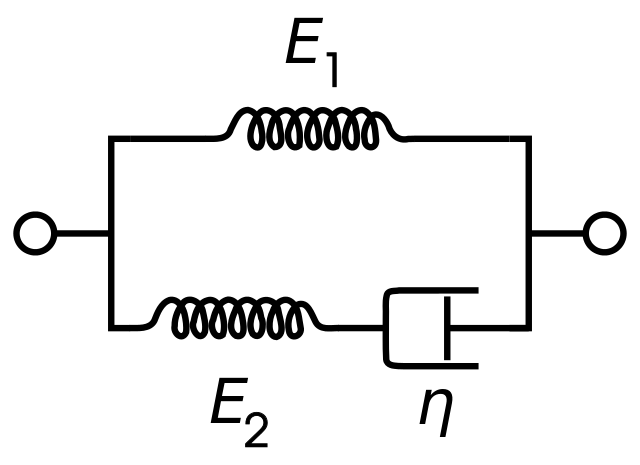
\includegraphics[width=0.6\textwidth]{images/Maxwell}
  \caption{The Maxwell form of the standard linear solid.}
  \label{fig:Maxwell}
\end{figure}

The stress and strain in the Maxwell element will be denoted by $\sigma_M$ and $\varepsilon_M$.
The stress and strain in the elastic element will be referred to as $\sigma_b$ and $\varepsilon_b$.
Since the Maxwell element is in parallel with the elastic element (isostrain):
\begin{equation}
  \varepsilon_M = \varepsilon_b = \varepsilon,
\end{equation}
where $\varepsilon$ is the total strain of the SLS.
The strain in the Maxwell element is the sum of the strains in the spring and dashpot element, i.e.,
$\varepsilon_a$ and $\varepsilon_d$, so
\begin{equation}\label{eq:varepsilonall}
  \varepsilon_a + \varepsilon_d = \varepsilon_b = \varepsilon.
\end{equation}
In the same time,
\begin{equation}
  \dot{\varepsilon}_a + \dot{\varepsilon}_d = \dot{\varepsilon}_b = \dot{\varepsilon}.
\end{equation}
The total stress for the overall system is the sum of the stresses in the individual branches:
\begin{equation}\label{eq:sigmaall}
  \sigma = \sigma_b + \sigma_M = E_b \varepsilon_b + \sigma_M = E_b \varepsilon + \sigma_M,
\end{equation}
where in the Maxwell element,
\begin{equation}
  \sigma_M = \sigma_a = \sigma_d.
\end{equation}
We assume
\begin{align}\label{eq:sigmaM}
  \sigma_a & = E_a \varepsilon_a,          \\
  \sigma_d & = 3 \eta \dot{\varepsilon}_d.
\end{align}
And bring \eqref{eq:sigmaM} into \eqref{eq:varepsilonall},
we get
\begin{equation}
  \varepsilon = \frac{ \sigma_a }{ E_a } + \varepsilon_d = \frac{ \sigma_M }{ E_a } + \varepsilon_d.
\end{equation}
Take derivative on both sides,
\begin{equation}\label{eq:epdot}
  \dot{\varepsilon} = \frac{ \dot{\sigma}_M }{ E_a } + \frac{ \sigma_M }{ 3 \eta }.
\end{equation}
Take \eqref{eq:sigmaall} into \eqref{eq:epdot},
\begin{equation}\label{eq:beforesimplify}
  \dot{\varepsilon} = \frac{ \dot{\sigma} - E_b \dot{\varepsilon} }{ E_a } + \frac{ \sigma - E_b \varepsilon }{ 3 \eta }.
\end{equation}
Simplify equation \eqref{eq:beforesimplify}, we get the equation of motion
\begin{equation}\label{eq:maineq}
  \begin{split}
    \bigg( 1 + \frac{ E_b }{ E_a } \bigg) \dot{\varepsilon} + \frac{ E_b }{ 3 \eta } \varepsilon &= \frac{ \dot{\sigma} }{ E_a } + \frac{ \sigma }{ 3 \eta },\\
    (E_a + E_b) \dot{\varepsilon} + \frac{ E_a E_b }{ 3 \eta } \varepsilon &= \dot{\sigma} + \frac{ E_a }{ 3 \eta } \sigma,\\
    \dot{\varepsilon} + A \varepsilon &= B \dot{\sigma} + C \sigma,
  \end{split}
\end{equation}
where $A = \dfrac{ E_a E_b }{ E_a + E_b } \dfrac{ 1 }{ 3 \eta }$, $B = \dfrac{ 1 }{ E_a + E_b }$, and $C = A / E_b$.

Now let's solve this equation. You can skip this if not interested.
We apply Laplace transform
\begin{equation}
  \mathcal{F}(s) = \mathcal{L}\{f(t)\} = \int_{0}^{\infty} e^{-s t} f(t) d t
\end{equation}
to \eqref{eq:maineq}. Since Laplace transform is a linear operator, i.e.,
\begin{equation}
  \mathcal{L}\{a f(t)+b g(t)\} = a F(s) + b G(s),
\end{equation}
we will have
\begin{equation}\label{eq:lapexpand}
  \mathcal{L}\{\dot{\varepsilon}\} + A \mathcal{L}\{\varepsilon\} = B \mathcal{L}\{\dot{\sigma}\} + C \mathcal{L}\{\sigma\}.
\end{equation}
Since $\sigma(t)$ is a step function $\sigma(t) = \sigma_0 H(t)$, with $H(t)$ be the Heaviside step function,
\begin{equation}
  \mathcal{L}\{\sigma\} = \frac{ \sigma_0 }{ s }.
\end{equation}
And since
\begin{equation}\label{eq:lapdot}
  \mathcal{L}\{\dot{f}(t)\} = s F(s)-f(0^{+}),
\end{equation}
here if $f(t)$ is bounded by
\begin{equation}
  | f(t) | = M e^{a t},
\end{equation}
where $M$ is a finite number, then \eqref{eq:lapdot} simplifies to
\begin{equation}
  \mathcal{L}\{\dot{f}(t)\} = s F(s) - f(0).
\end{equation}
Of course in real world, $\varepsilon$ and $\sigma$ are finite, so
\begin{align}
  \mathcal{L}\{\dot{\sigma}\}      & = s \frac{ \sigma_0 }{ s } - \sigma(0) = 0,      \\
  \mathcal{L}\{\dot{\varepsilon}\} & = s \mathcal{L}\{\varepsilon\} - \varepsilon(0).
\end{align}
So \eqref{eq:lapexpand} simplifies to
\begin{equation}
  C \frac{ \sigma_0 }{ s } = s \mathcal{L}\{\varepsilon\} - \varepsilon(0) + A \mathcal{L}\{\varepsilon\},
\end{equation}
so
\begin{equation}\label{eq:transformed}
  \mathcal{L}\{\varepsilon\} = \frac{ C \frac{ \sigma_0 }{ s } + \varepsilon(0) }{ s + A }.
\end{equation}
Now what's $\varepsilon(0)$? Definitely it is a constant. Let's call it $\varepsilon_0$.

So apply inverse Laplace transform to \eqref{eq:transformed}, we have
\begin{equation}
  \varepsilon(t) = \frac{(E_b \varepsilon_0-\sigma_0) e^{-\frac{E_a E_b t}{3 \eta (E_a + E_b)}}}{E_b}+\frac{\sigma_0}{E_b},
\end{equation}
where $E_b \varepsilon_0 \leq \sigma_0$ since $\sigma_M(0) \geq 0$.
When $t \rightarrow \infty$, we can clearly see that
\begin{equation}
  \varepsilon(\infty) = \frac{\sigma_0}{E_b},
\end{equation}
as is expected.

So
\begin{equation}
  E(t) = \frac{ \varepsilon(t) }{ \sigma_0 } = \frac{(E_b \varepsilon_0-\sigma_0) e^{-\frac{E_a E_b t}{3 \eta (E_a + E_b)}}}{E_b \sigma_0}+\frac{1}{E_b},
\end{equation}
\begin{figure}[h]
  \centering
  \includegraphics[width=0.6\textwidth]{images/8_3}
  \caption{$\varepsilon(t)$, with different intial $\varepsilon_0$, where $E_a = 1$, $E_b = 3$, $\eta = 1$, $\sigma_0 = 10$.}
  \label{fig:question_8_3}
\end{figure}

See figure \ref{fig:question_8_3} for reference.

\subsection{8.4}
The elongation of a cylinder of slightly viscoelastic material is found to be
$1\%$ greater for a step stress $\sigma_0$ measured after \SI{1}{\day} compared with after \SI{100}{\femto\second}.
If the viscoelasticity of the cylinder is dominated by a single defect
with a single relaxation time, what will be the \emph{shortest} time for a spring made from this
material set into free vibration to decay to $10\%$ of its initial amplitude,
if measurements are taken for a full range of masses applied to the end of the spring?

\textbf{Solutions:}

From the problem statement:
\begin{equation}
  \varepsilon(\SI{86400}{\second}) = 1.01 \varepsilon(\SI{1e-13}{\second}).
\end{equation}
Treating our slightly viscoelastic solid as a standard-linear solid:
\begin{equation}
  \varepsilon_{R} = 1.01 \varepsilon_{U}.
\end{equation}
For an applied step stress $\sigma_{0} = E \varepsilon$,
\begin{equation}
  E_{R}^{-1} = 1.01 E_{U}^{-1}.
\end{equation}
This form compares well with equation $(8.91)$. Hence, we can use the sinusoidal response in the limit of
small difference between the relaxed and unrelexed moduli in order to estaimate $Q$, where
\begin{equation}
  \Delta = 0.01.
\end{equation}
So,
\begin{align}
  \big( Q^{-1} \big)_\text{max} & = \frac{ \Delta }{ 2 } = 0.005, \\
  Q_\text{min}                  & = 200.
\end{align}
Unfortunately, we can’t go much farther with the problem. There was a slight error in the problem
statement. It turns out a resonance frequency, or some related quantity, needs to be provided in order
to calculate $\tau_C$. Recall:
\begin{equation}
  \tau = \frac{ 2 \pi }{ \omega_0 },
\end{equation}
and
\begin{equation}
  \tau_C = \frac{ Q \tau }{ \pi }.
\end{equation}
Then using $\tau_C$ we could easily find the minimum decay-time for a spring made of the this material,
set into free-vibration, to decay to $10\%$ of its original amplitude. As an aside, please note that the
minimum decay time occurs at the value for which quality factor of the resonance is minimized. Less
sharply peaked resonances, hence lower quality factors, correspond to more loss (dissipation) in the
system. This occurs when $\omega \tau = 1$. Where the frequency dependent behavior of the quality factor can
be determined from:
\begin{equation}
  Q^{-1} = \big( Q^{-1} \big)_\text{max} \frac{ 2 \omega \tau }{ 1 + \omega^2 \tau^2 }.
\end{equation}
Back to the problem at hand. The shortest decay-time for a spring made of the this material, set into
free-vibration, to decay to $10\%$ of its original amplitude is:
\begin{equation}
  \frac{ u(N) }{ u_0 } = e^{-\frac{ \tau }{ \tau_C }} = 0.1.
\end{equation}


\subsection{8.5}
The notes on a piano span a range from \SI{27.5}{\hertz} to \SI{4186}{\hertz}.
The A keys are tuned to \SI{440}{\hertz} for A4, with each octave doubling in frequency
in the following sequence: 27.5, 55, 110, 220, 440, 880, 1760, 3520 Hz for A1-A8 on
the keyboard.  Plot (using python) as a function of frequency over A0-A7 \emph{the sustain time}
for a given note struck on the piano, defined as the time needed for the volume (square of amplitude)
to decay to $1/e$ its initial value.  Use a logarithmic scale for the frequency. Make your estimate
\begin{enumerate}[a)]
  \item assuming that the $Q$ value for the oscillation is that for A4 as calculated in the lectures.

        \textbf{Solutions:}

        From section $8.4.3$:
        \begin{align}
          \tau_0   & = \SI{1.89e-15}{\second},        \\
          \Delta H & = \SI{83700}{\joule \per \mole}.
        \end{align}
        First assuming that the $Q$ value for the oscillation is that for A4 as calculated in the lectures:
        \begin{equation}
          Q^{-1} = \big( Q^{-1} \big)_\text{max} \sech \bigg( \ln(\omega \tau_0) + \frac{ \Delta H }{ R T } \bigg),
        \end{equation}
        where
        \begin{equation}
          \big( Q^{-1} \big)_\text{max} = \frac{ \num{5.4e-5} }{ \num{5.1e-4} } = 0.106,
        \end{equation}
        and $R = 8.314$, $T = 295$.
  \item taking into account the frequency dependence of $Q$ expected for piano wire. Does the result seem reasonable?

        \textbf{Solutions:}
        Taking into account the frequency dependence of $Q$:
        \begin{equation}
          \tau_C = \frac{ Q }{ 2 \pi \nu } = \frac{ 1 }{ 0.106 \times 2 \pi \nu } \cosh \bigg( \ln(2 \pi \nu \tau_0) + \frac{ \Delta H }{ R T } \bigg).
        \end{equation}

        Now we can plot for A1-A8 on the keyboard, as figure \ref{fig:tauc} shows.
        \begin{figure}[h]
          \centering
          \includegraphics[width=0.7\textwidth]{./images/8_5}
          \caption{$\tau_C$ VS $\nu$, in log scale.}
          \label{fig:tauc}
        \end{figure}

        This answer does not seem reasonable given that we would expect higher notes to
        ring longer than the lower notes. Our answer shows very little differnce in
        magnitude between the characteristic times for A1-A8.
        However, this answer does not account for differing lengths of the piano wires
        used for the varying notes amongst other things.

\end{enumerate}




% \bibliographystyle{unsrt}
% \bibliography{ref}

% --------------------------------------------------------------
%     You don't have to mess with anything below this line.
% --------------------------------------------------------------

\end{document}